Chaque joueur peut choisir son contrôleur de jeu via les options du menu. Il a le choix entre ces différents périphériques :

\begin{itemize}
	\item le clavier
	\item Joystick
	\item wiimote
\end{itemize}
	
	
\subsubsection{Clavier}
Il est possible de paramétrer les différentes commandes du jeu en passant par le menu.

Par défaut les commandes du jeu sont les suivantes :

\begin{center}
	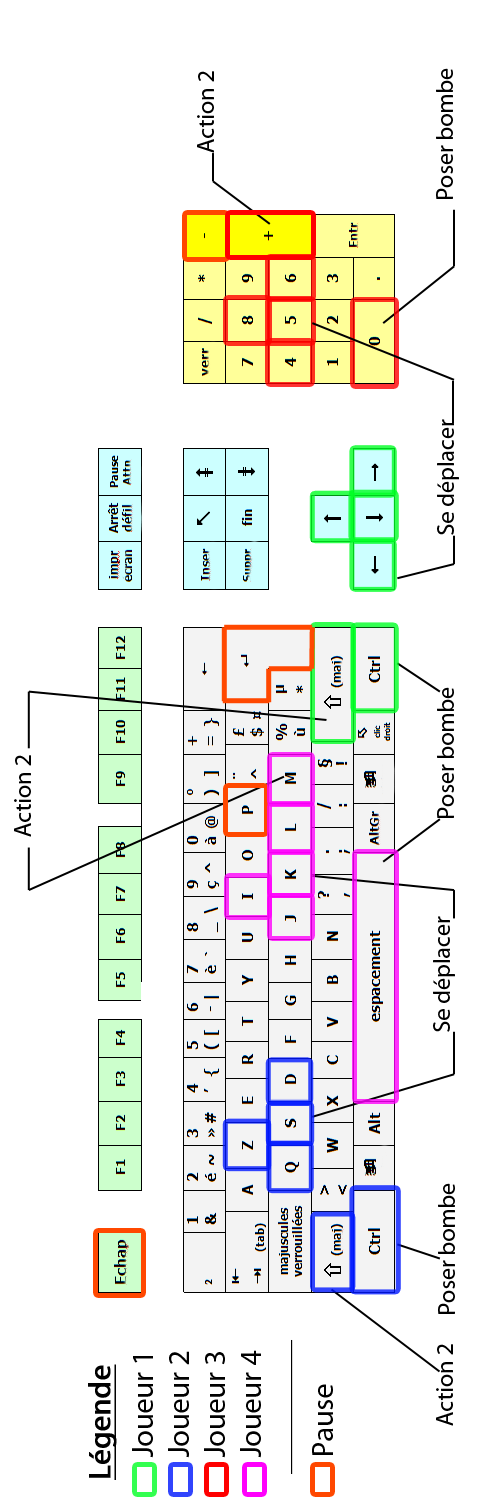
\includegraphics[height=550pt]{images/clavier}
\end{center}

\subsubsection{Joystick}
La prise en charge des contrôleurs de jeu PC de type Joystick se fait par l'intermédiaire de la librairie SFML.

Comme le clavier, il est possible de paramétrer les différentes commandes du jeu en passant par le menu.

Par défaut les commandes du jeu sont les suivantes :

\begin{center}
	\begin{tabular}{|c|c|}
		\hline
			\rowcolor{blueTab}
			\textbf{Action} & \textbf{Touche(s)} \\
		\hline
		Se déplacer & Pad directionnel \\
		\hline
		Poser une bombe & Bouton 1\\
		\hline
		Action 2 & Bouton 2\\
		\hline
	\end{tabular}
\end{center}


\subsubsection{Wiimote}
La prise en charge d'un contrôleur de type Wiimote se fait par l'intermédiaire de la librairie Wiiusecpp. Cette librairie sous licence GNU GPLv3 et GNU LGPLv3 (non commercial) est codée en langage C++ et est principalement basée sur la librairie Wiiuse. La librairie est disponible pour les systèmes d'exploitation Linux et Windows.

Le jeu ne requiert pas l'utilisation du nunchuck.

Les commandes de jeu sont les suivantes et ne peuvent être modifiées :

\begin{center}
	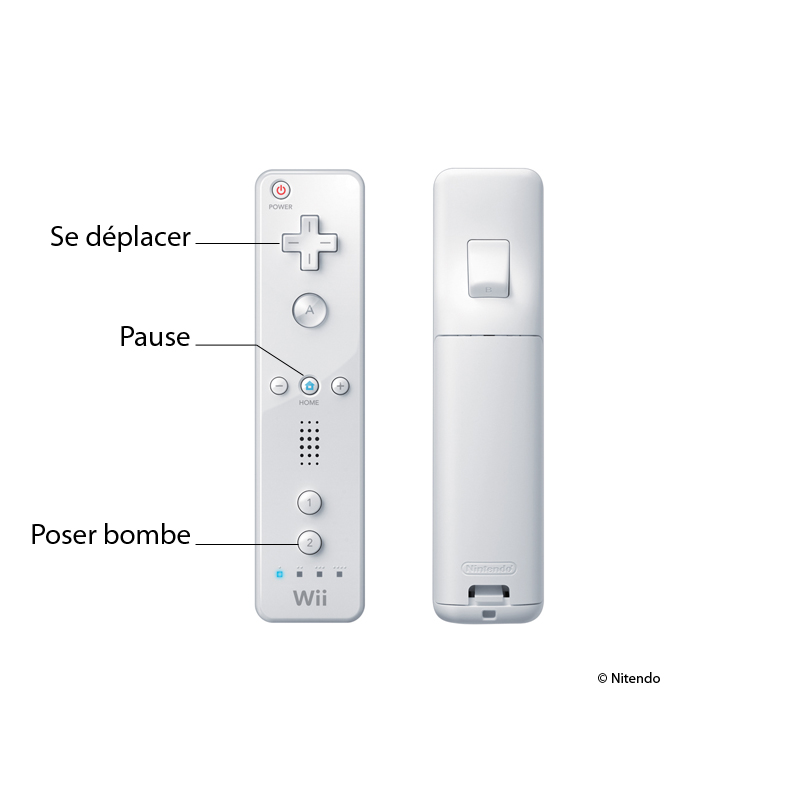
\includegraphics[scale=1.7]{images/wiimote}
\end{center}